\documentclass[12pt]{article}

\usepackage{graphicx}
\usepackage{listings}
\usepackage{hyperref}
\usepackage{float}
\usepackage{enumitem}

\graphicspath{ {./images/} }

\oddsidemargin 0mm
\evensidemargin 0mm
\textwidth 160mm
\textheight 200mm

\pagestyle {plain}
\pagenumbering{arabic}

\newcounter{stepnum}

\title{CS/SE 2XC3 Lab 4 Report}
\author{
  Glotov, Oleg\\ L03, 400174037\\
  \texttt{glotovo@mcmaster.ca}
  \and
  Willson, Emma\\ L02, 400309856\\
  \texttt{willsone@mcmaster.ca}
  }
\date{\today}

\begin{document}

\maketitle

This report includes the main observations that we found in this week's lab, along with the analysis of our results.

\newpage 
\section{Mergesort}
In this section, we discuss the complexities of various implementations of merge sort, conduct experiments to investigate their performance, and analyze the results of those experiments.
\subsection{Experimental Method}
The method used to measure the performance of each sorting function was the same as the method used for lab 3. The “timeit” library was used to measure the runtime which was then exported into a csv file and subsequently analyzed in excel. The sample size for each sorting implementation were multiples of 10, increasing to a list size of a 1 000 000. For each sample size, an implementation was tested 5 times and the results averaged. For each trial, a new random list was generated. 

\subsection{Bottom-up}
Implement a function mergesort\_bottom(L) which takes a single list as input and sorts
that list L. Implement a helper function merge_bottom(L, start, mid, end). This should merge
the interval [start:end] assuming [start:mid] and [mid:end] are sorted. The ex-
act inclusive/exclusive decisions for the intervals are left up to you. As long as your
mergesort\_bottom(L) works. Your functions should not be recursive in anyway. Loops only. Note, in Figure 2 the length of the list is conveniently a power of 2, this may not be the
case. You will have to resolve this in some way. Compare this bottom-up implementation to the one I gave you in lab4.py

In our implementation of bottom-up mergesort, we treat the input list as if it were already divided into 1 element lists and iteratively merge pairs of lists until the sorting window is the same size as the input. Since this approach assumes that the size of the input is a power of 2, we maintain a sublist of remainders that is left unmerged until the last step. 

Using the experimental method described in section 1.1, I generated timing data for  \verb+mergesort()+ and \verb+mergesort\_bottom()+ with list lengths ranging from 10 to 1 000 000. I used the provided function \verb+create\_random\_list()+ to generate each trial list. These results are shown in the graph below. 

\begin{figure}[H]
\centering
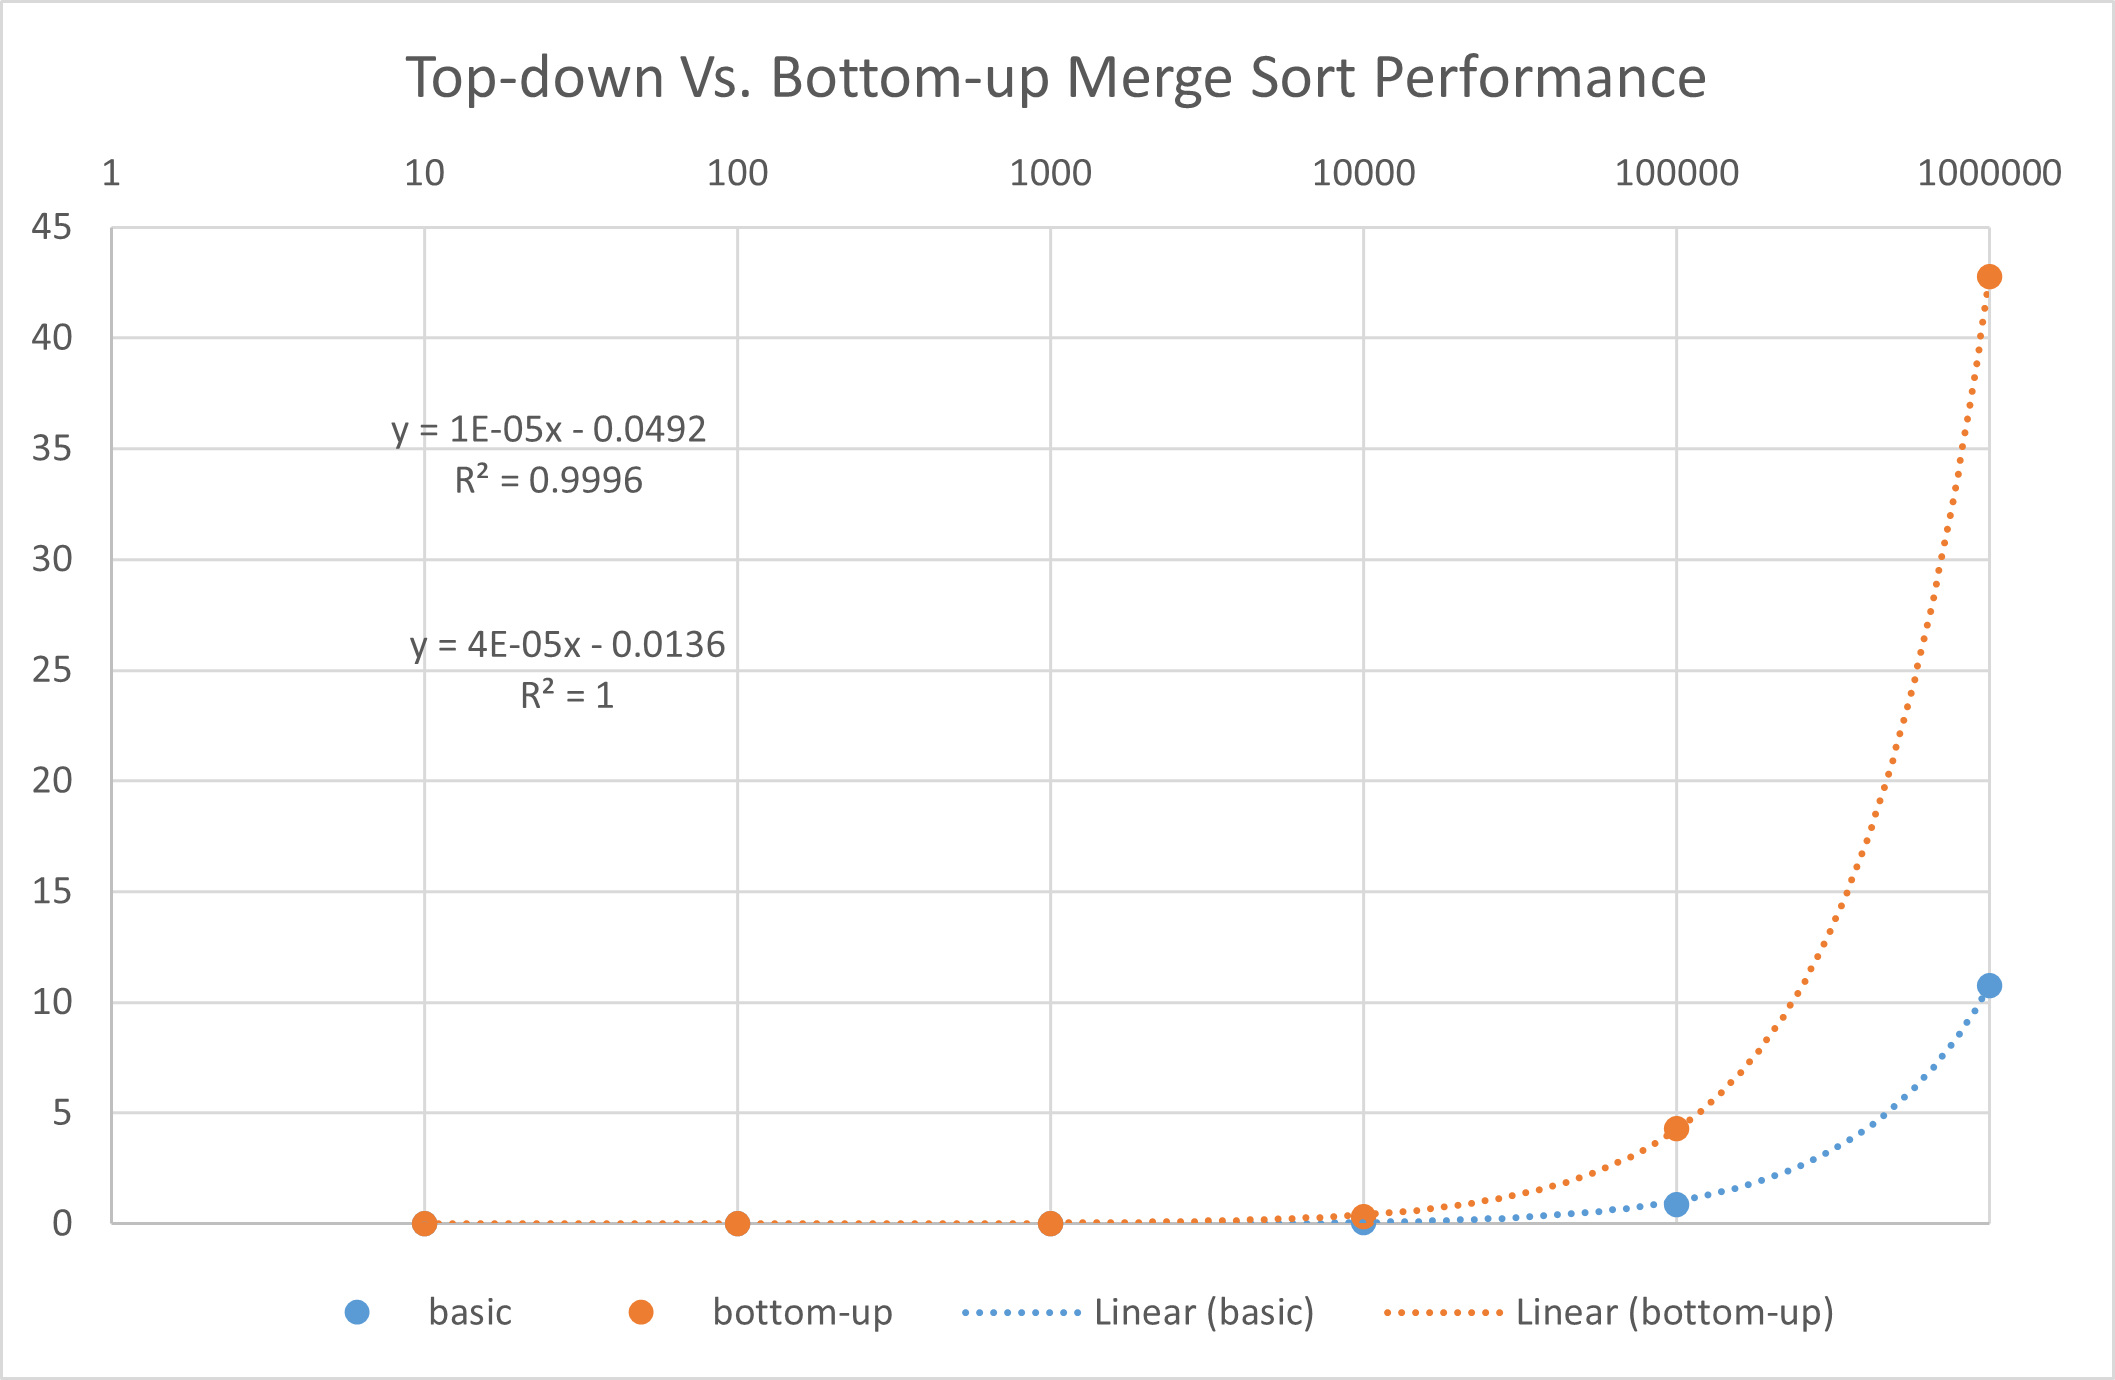
\includegraphics[width=0.9\textwidth,height=\textheight,keepaspectratio]{bottom_up}
\caption{performance of top-down compared to bottom-up implementation}
\label{Figure: i1}
\end{figure}
\noindent The two implementations are similar in performance in that they both seem to follow a linear trendline. However, the bottom-up implementation is slower than top-down. Right now, we have a linear trendline for both implementations, but we can check if the performances of these functions are in $\Theta(n)$ or $\Theta(n\log{n})$ by graphing $T(n)/n$.

\begin{figure}[H]
\centering
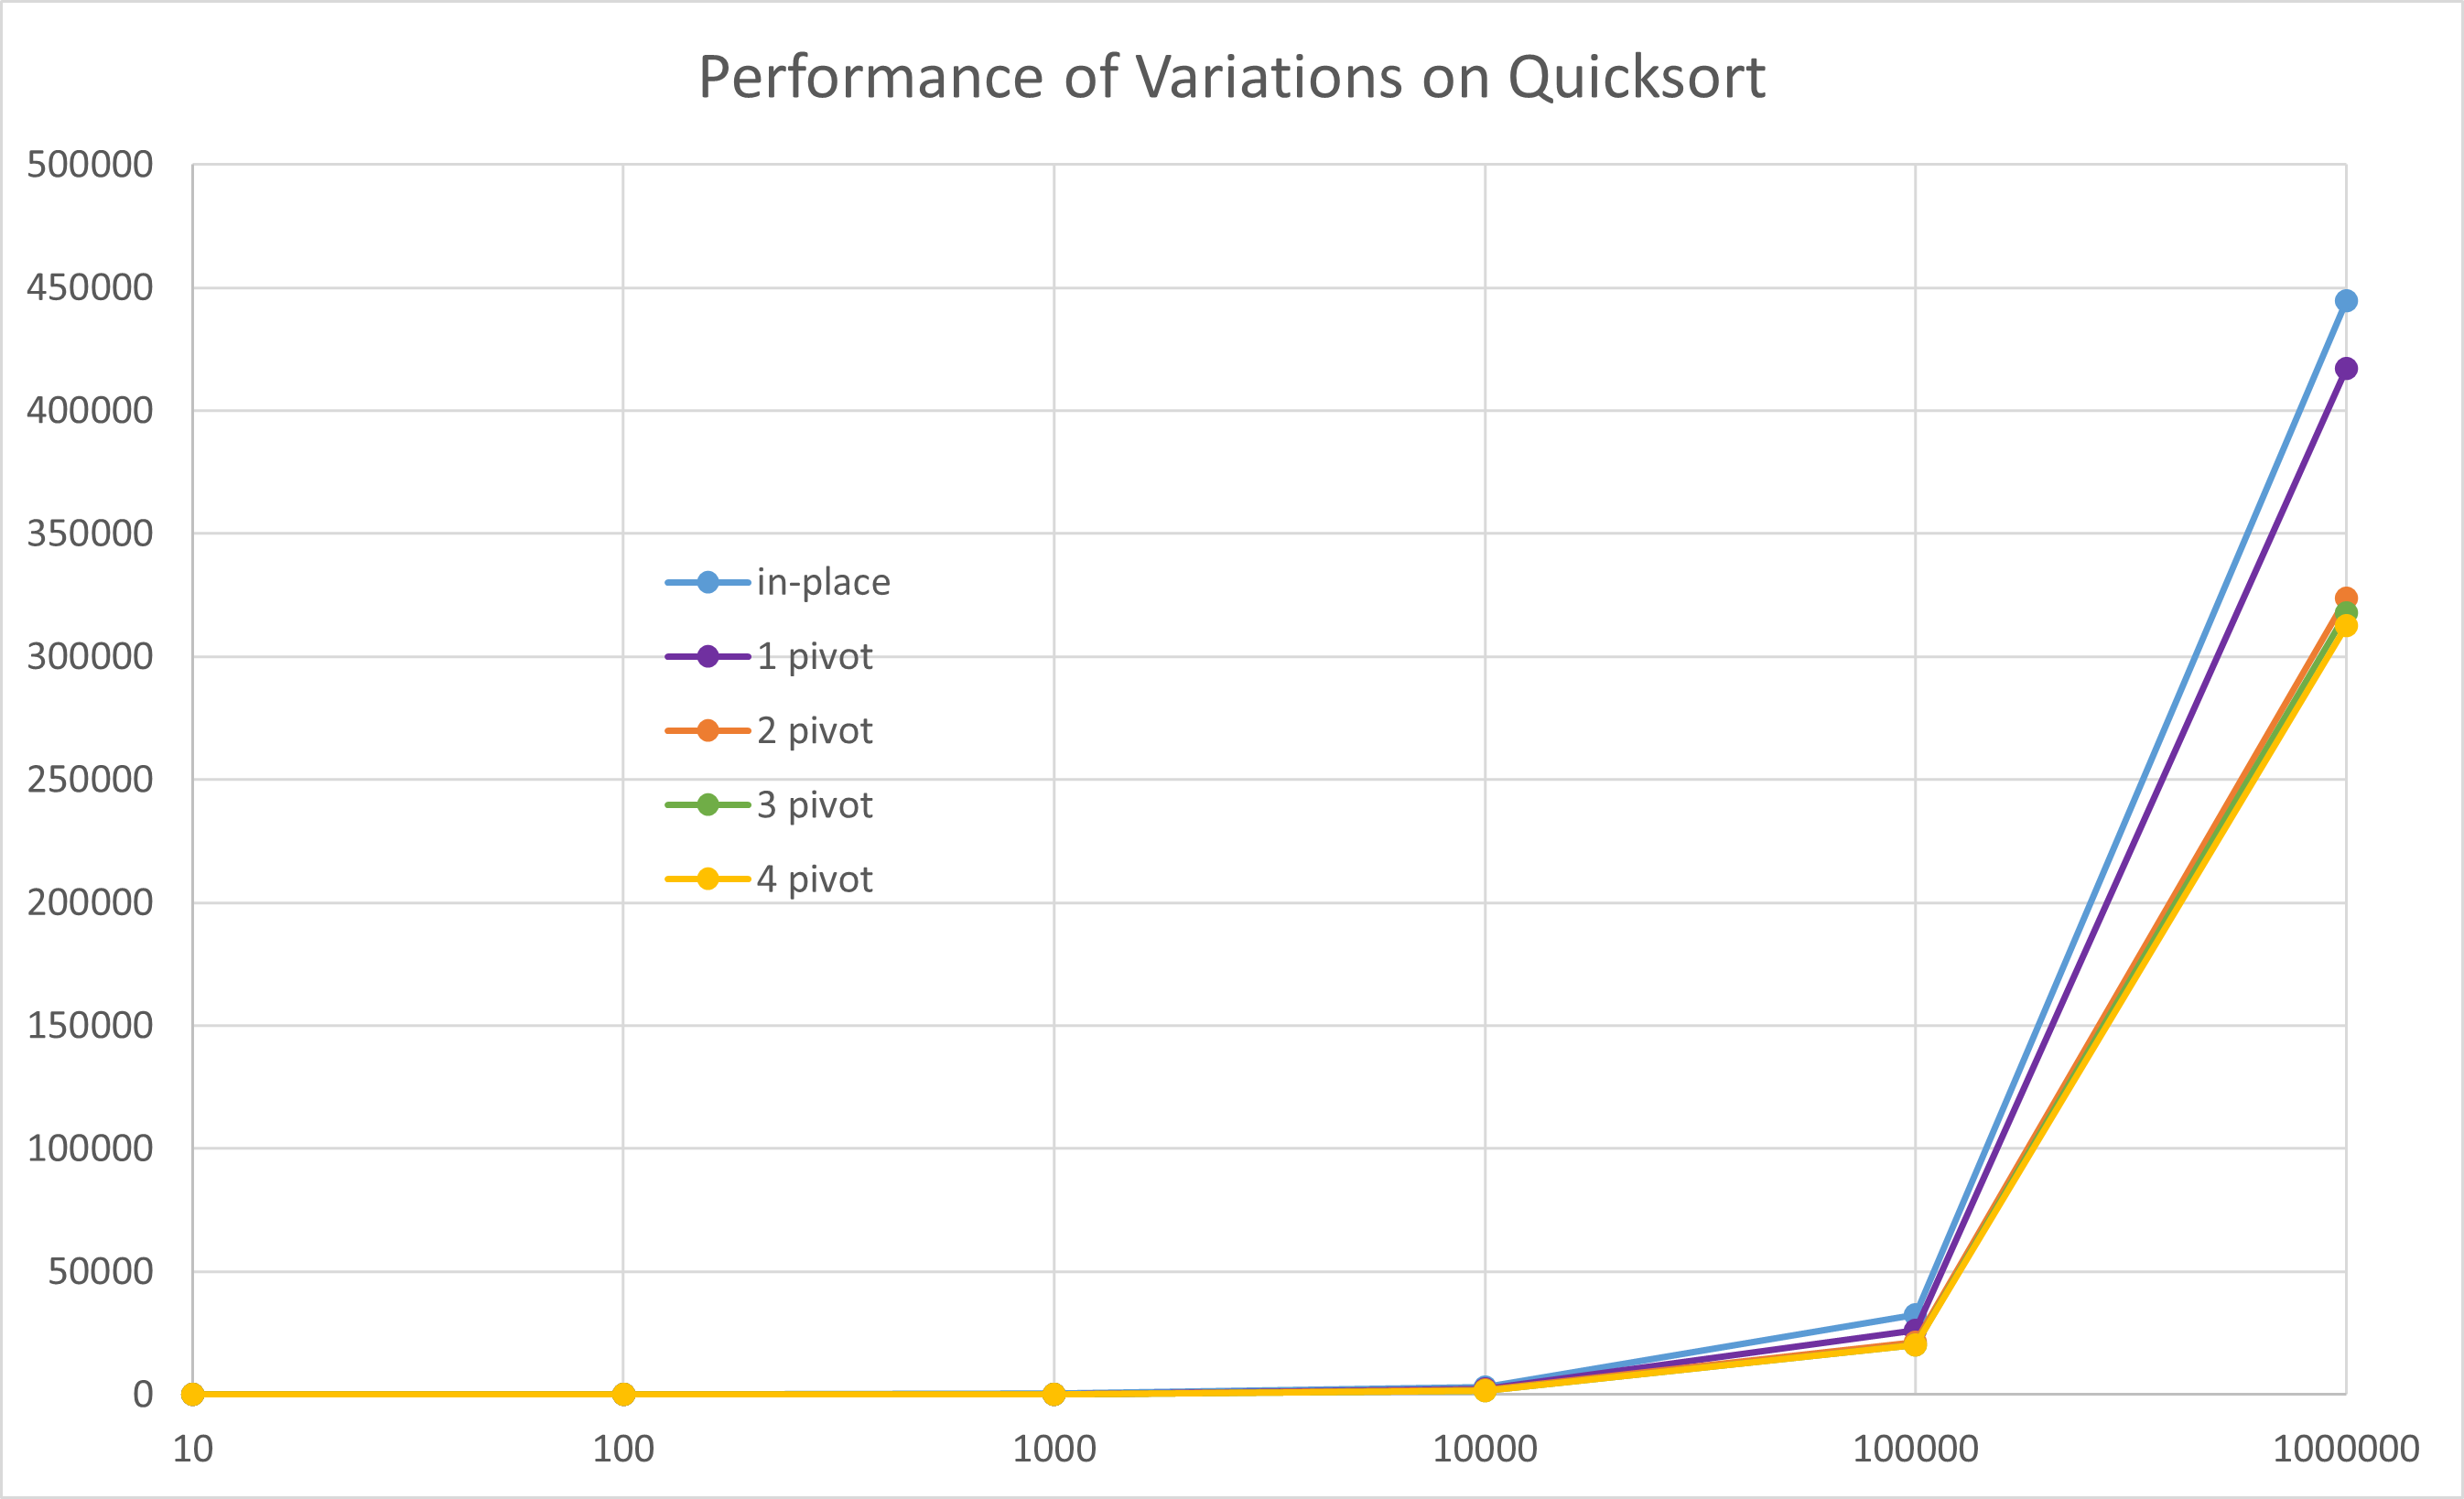
\includegraphics[width=0.9\textwidth,height=\textheight,keepaspectratio]{multi_pivot}
\caption{performance of all five implementations}
\label{Figure: m1}
\end{figure}

In practice, I would most likely use the traditional implementation because it is faster. An occasion when I might want to use the in-place implementation is if I was sorting a list that takes up a lot of space and did not want to take up twice as much space to do so. That list might have a very big number of elements, or very big individual elements. 

\subsection{Multi-Pivot Quicksort}
I used the same experimental method from 1.1 to test my implementations of multi-pivot quicksort. I generated timing data for \verb+my_quicksort()+, \verb+dual_pivot_quicksort()+, \verb+tri_pivot_quicksort()+, and \verb+quad_pivot_quicksort()+. I analyzed and graphed the data, which is shown below.



The data clearly shows a 20 to 25\% improvement in runtime between a 1 and 2 pivot quicksort. Further increases in the number of pivots only improved the runtime by 1 to 2\% which is insignificant. For further experiments I would recommend following the example of Java developers and using the 2-pivot quicksort as the default quicksort, similar to how it is used as the default sorting algorithm in Java 7. For the rest of this lab, we use 2-pivot quicksort as our default quicksort.

\subsection{Worst Case}
The worst case performance for quicksort occurs when the chosen pivot is always either the smallest or the largest element. In the case of a dual-pivot quicksort, the worst case occurs when both pivots are either the two largest elements, the two smallest, or the largest and smallest elements. Our quicksort picks the first and last elements of the list as the pivots, so an already-sorted list would be the worst-case input. 

\footnotesize
\begin{verbatim}
def dual_pivot_quicksort(L):
    copy = quicksort_2pivot(L)
    for i in range(len(L)):
        L[i] = copy[i]

def quicksort_2pivot(L):
    if len(L) < 2:
        return L
    pivotL = L[0]
    pivotR = L[-1]
    if (pivotL >= pivotR):
        temp = pivotL
        pivotL = pivotR
        pivotR = temp
    left, right, mid = [], [], []
    for num in L[1:-1]:
        if num < pivotL:
            left.append(num)
        elif pivotL <= num and num <= pivotR:
            mid.append(num)
        else:
            right.append(num)
    final = quicksort_2pivot(left) + [pivotL] + quicksort_2pivot(mid) + [pivotR] + quicksort_2pivot(right)
    return final
\end{verbatim}
\normalsize

To test the worst case performance, I generated a random list and a reverse-sorted list for each trial and then recorded the time taken to sort it using my dual-pivot quicksort. To generate these lists, I used \verb+create_random_list()+ and then the built-in \verb+sort()+ and \verb+reverse()+ Python functions. When collecting performance data for this experiment, I tried to follow the same steps as in the previous experiments. However, for data points after input size 1000, I recieved a maximum recursion depth error. The maximum recursion depth for the version of Python that I am running is 1000 [1]. This means that, at input size 10 000, our worst case quicksort run should have reached over 1000 recursive calls. Due to the way that the function selects pivots, a sorted list would only be separated into one middle list and 2 outer pivots with each recursive call. Then, the number of recursive calls would be $\frac{n}{2}$, where $n$ is the input size. 
Consequently, I only collected data up to input size 1000 for the worst case test. The results of this experiment are shown in the graph below. 

\begin{figure}[H]
\centering
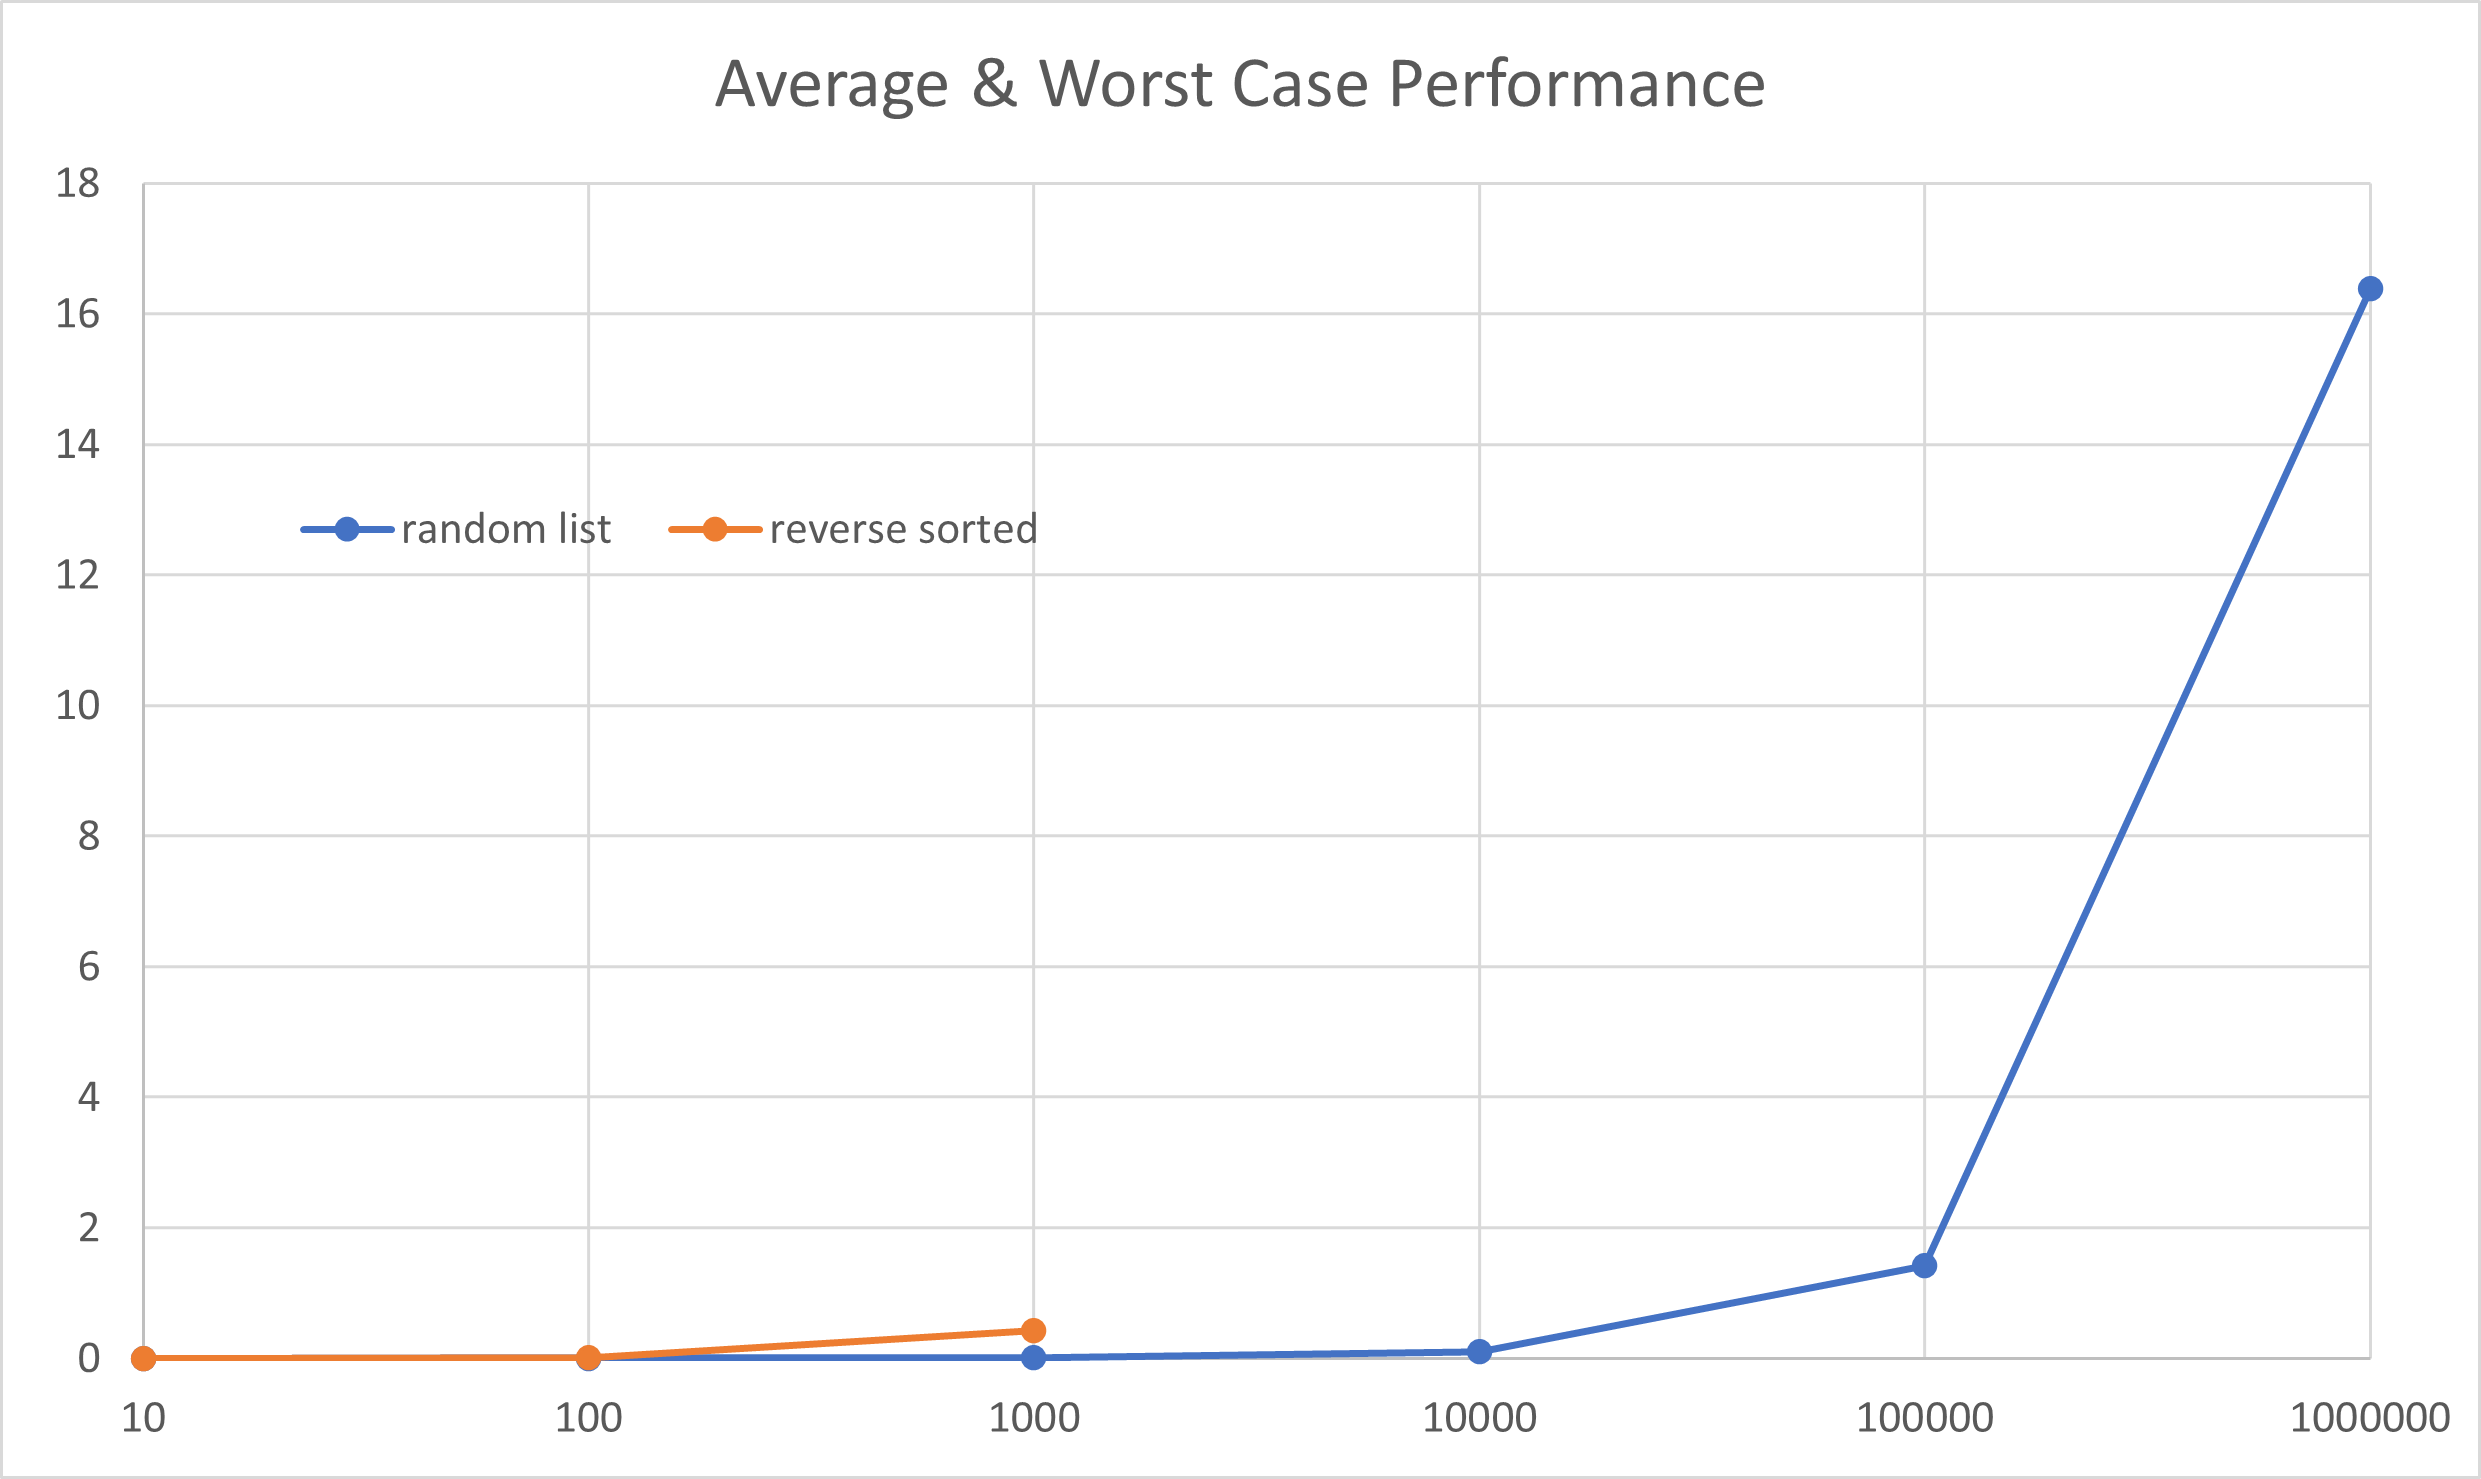
\includegraphics[width=0.9\textwidth,height=\textheight,keepaspectratio]{worst_case}
\caption{average and worst-case performance of dual-pivot quicksort}
\label{Figure: w1}
\end{figure}

\noindent There is not a lot of data for the worst case input, but it is clear from the graph and the maximum recursion depth error that the complexity is increasing at a much greater rate than the average case with respect to \verb+n+. With each recursive call, each non-pivot element in \verb+L+ is compared to \verb+pivotL+ and \verb+pivotR+. Since this is the worst case and each non-pivot element is going to be between the two pivots, only the \verb+mid+ list is passed in the recursive call, with a length of $n-2$. The number of compares $= 2*((n-2) + (n-4) + (n-6) + ... + 4 + 2) = n*(n-2)$, which is in $O(n^2)$. This is worse than the average case, which runs in $O(n\log{n})$ [2].

The \verb+create_near_sorted_list()+ function takes an integer \verb+i+ and a float \verb+factor+ and generates a list of random numbers of size \verb+i+. It sorts the list and then performs \verb+i*factor+ swaps on randomly selected elements in the list, finally returning the partially sorted list. The smaller the \verb+factor+, the fewer swaps are performed. When the list is close to sorted, I would expect the bubble and insertion sorts to perform better than our quicksort implementation. This is because the implementation of bubble sort that we use has a swap counter that checks if any swaps need to be performed. If the input list is already sorted, the function can detect this after the first loop. This allows the loops to terminate before visiting every element, which is better for near-sorted lists. This implementation of bubble sort is shown below.

\footnotesize
\begin{verbatim}
def bubble_sort_opt3(L):
    for i in range(len(L)):
        swaps = 0
        for j in range(len(L) - 1 - i):
            if L[j] > L[j+1]:
                swap(L, j, j+1)
                swaps += 1
        if swaps == 0:
            return
\end{verbatim}
\normalsize

\noindent Insertion sort is similar to this implementation of bubble sort in that it can quickly check if the input list is already in order. Insertion sort simply iterates through the list and, if an element is out of place, it backtracks in order to find the proper place for it. I expect bubble and insertion sort to perform better than quicksort for near-sorted lists because they are optimal for these kinds of inputs.

For my experiment, I chose to test my dual-pivot quicksort, optimized bubble sort, insertion sort, and selection sort on lists of length 1000. These lists we randomly generated, much like the method describe in section 1.1, except in this experiment they were generated using the \verb+create_near_sorted_list()+ function, with \verb+factor+ values ranging from 0.0001 to 1000. I chose to focus the \verb+factor+ values around this range because when \verb+factor+ = 0.001, only one swap is performed. When \verb+factor+ = 1, 1000 swaps are performed, so the list should be completely randomized again. I generated five trials per data point and took the average of them, as usual. This data is shown in the graph below.

\begin{figure}[H]
\centering
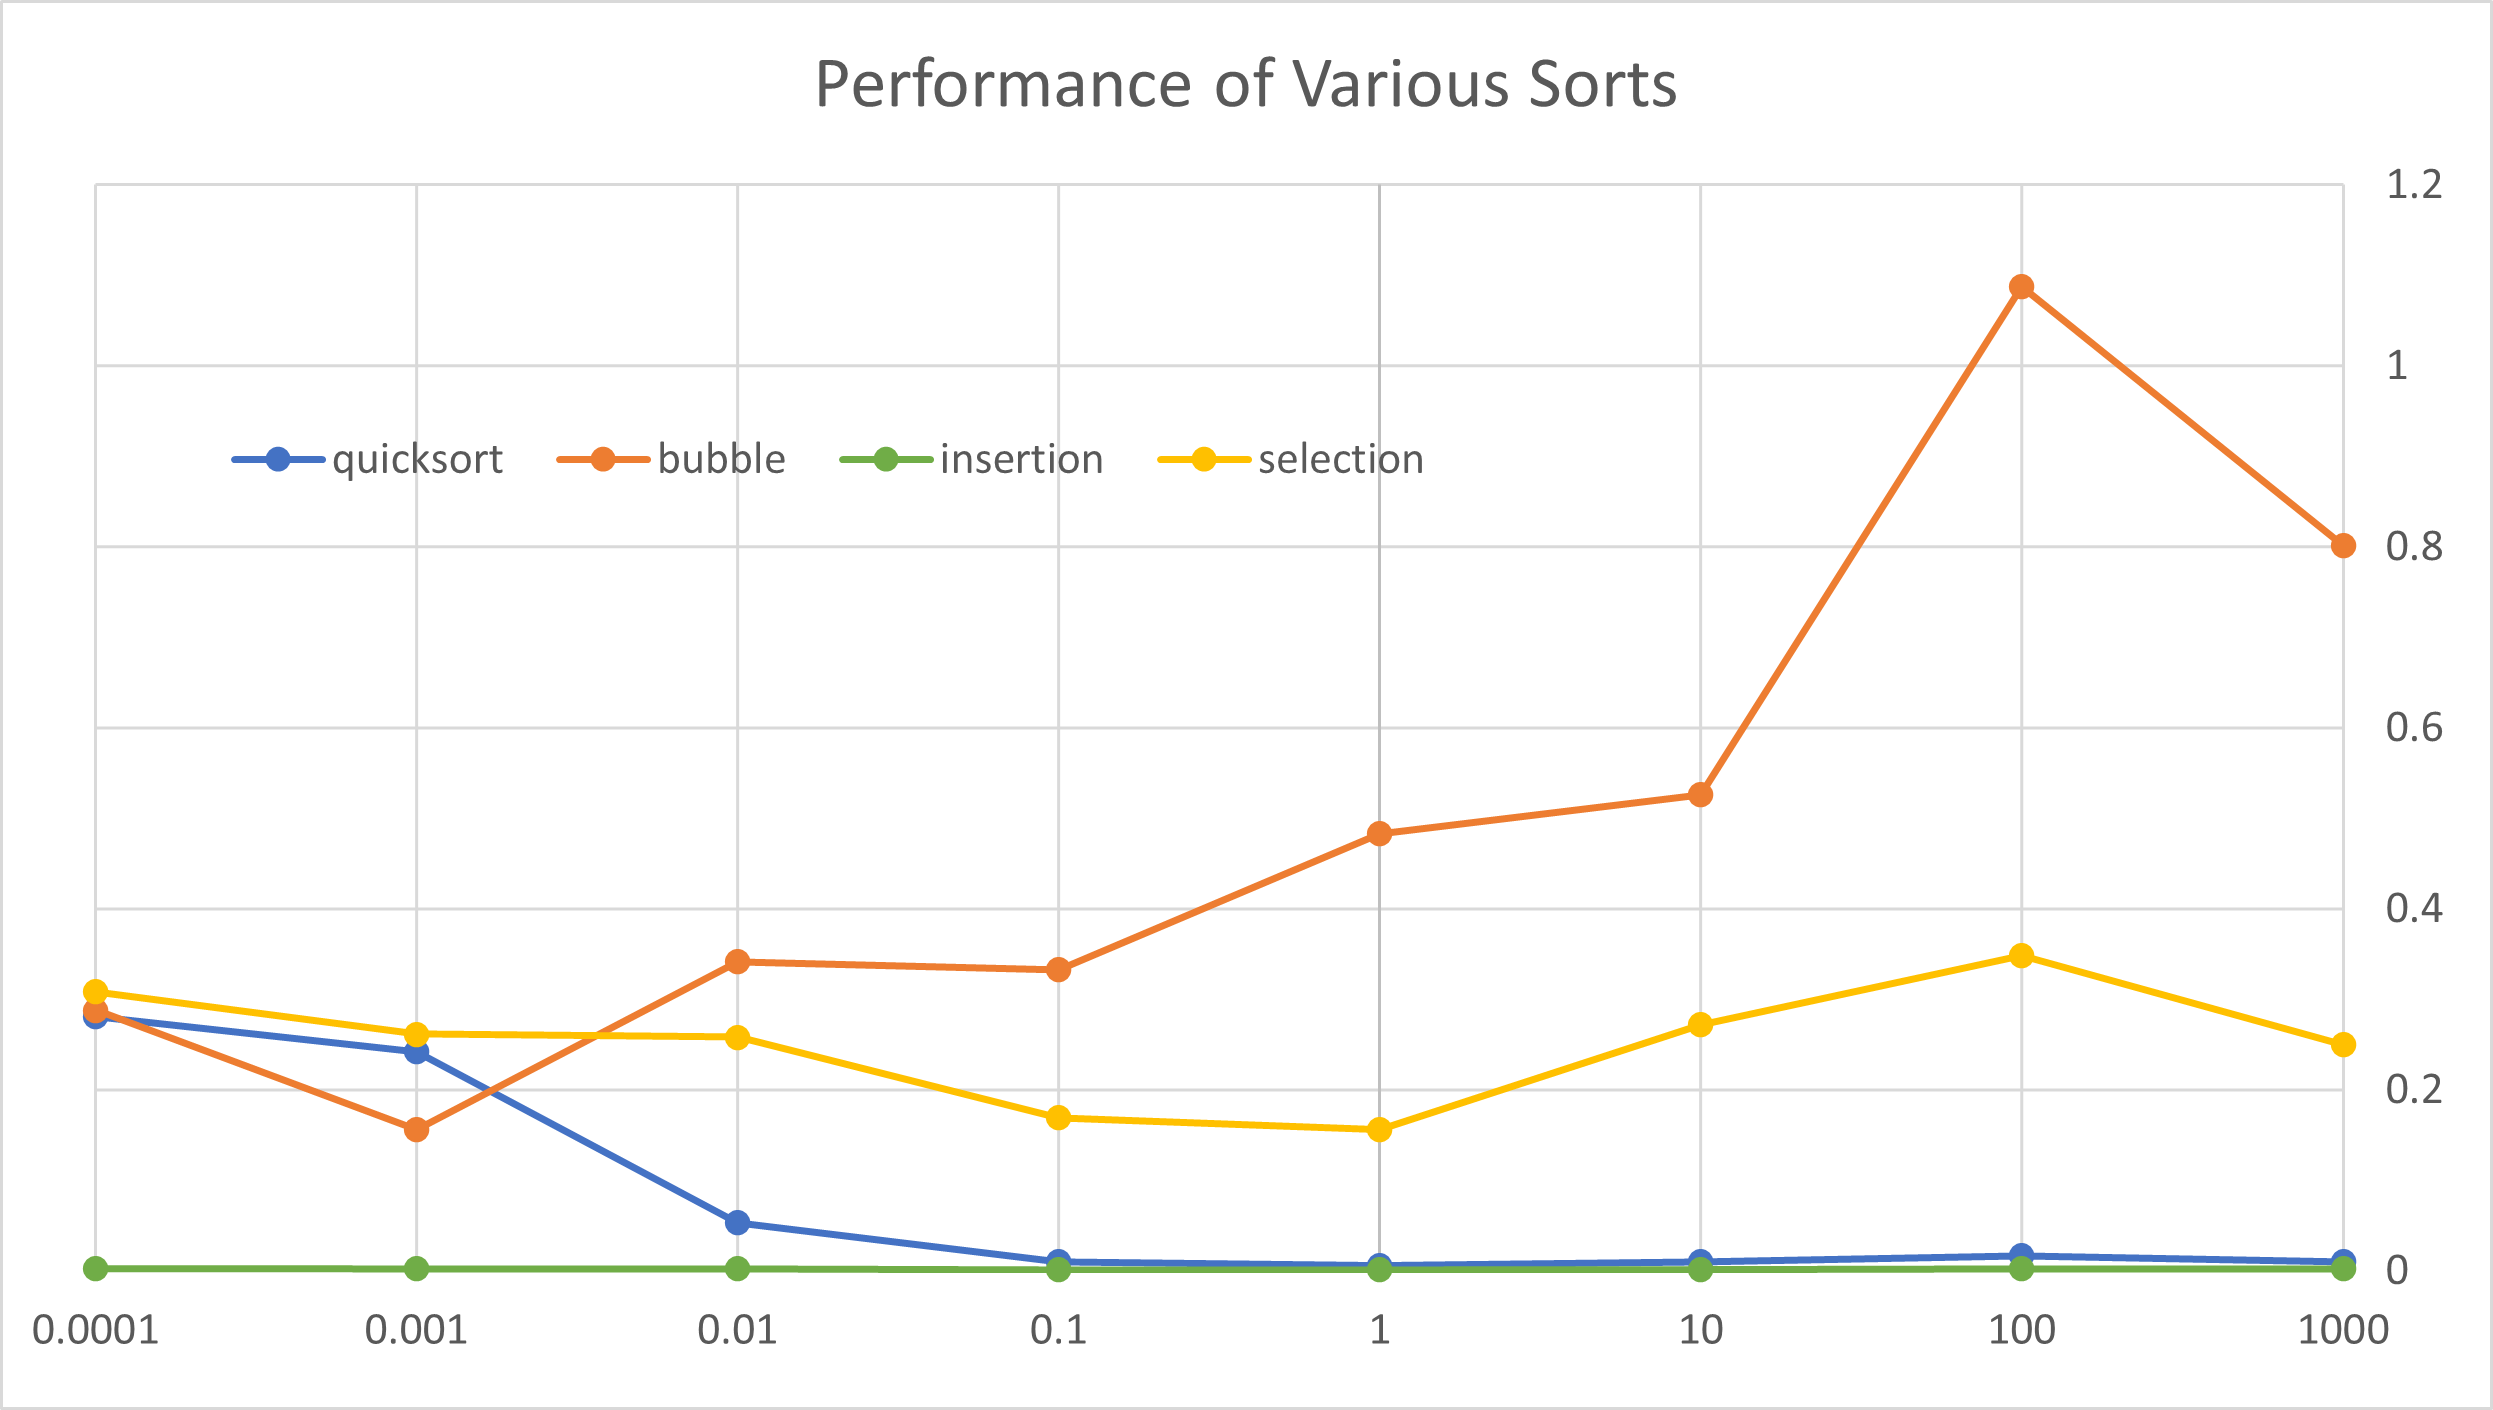
\includegraphics[width=0.9\textwidth,height=\textheight,keepaspectratio]{sorted_factor}
\caption{performance of various sorts on partially sorted lists}
\label{Figure: w2}
\end{figure}

\noindent As we can see in the graph, bubble and insertion sort perform better than quicksort for sorted-factor values of 0.001 and smaller. This means that between 10 and 100 swaps, bubble sort's time complexity dramatically increases in comparison to quicksort. Insertion sort performs better than quicksort for all the values that were tested. These elemantary sorts' performance is probably due to their abilities to detect an already sorted list, as well as the fact that these implementations are non-recursive. Meanwhile, our quicksort does not check if the input list is already sorted, yielding worst-case behaviour. Also quicksort is recursive, resulting in additional overhead.

\subsection{Small Lists}

As an improvement for quicksort, we decided to combine the average case efficiency of quicksort with the speed insertion sort handles nearly sorted arrays. We noticed that insertion sort is much quicker than quicksort for very small array sizes. Our \verb+final_sort()+ algorithm implements insertion sort on partitions with less than 10 elements. To further increase performance we employed a median-of-3 approach to pivot selection. The common pathologies $O(n^2)$ of sorted/reverse sorted inputs are mitigated with this improvement. 

When using a median-of-3 approach it is important to also sort the three elements when picking the median. This approach would ensure fair pivot selection in all recursive calls and lead to a more evenly partitioned array.

\footnotesize
\begin{verbatim}
pivot = median(array[0],array[-1],array[int(len(array)/2)])

[...]

def biggest(a,b,c):
    return bigger(a,bigger(b,c))

def bigger(a,b):
    if a > b:
        return a
    else:
        return b

def median(a,b,c):
    x = biggest(a,b,c)
    if x == a:
        return bigger(b,c)
    if x == b:
        return bigger(a,c)
    else:
        return bigger(a,b)
\end{verbatim}
\normalsize


\section{Conclusion}
 In this lab, we explored different implementations of quicksort. We designed and tested the performances of in-place and multi-pivot quicksorts. Our analysis shows that in-place sorting saves memory usage, but it does not improve time complexity. We also found that adding pivots to the quicksort algorithm improves time complexity, but as more pivots are added, that improvement becomes less significant. We determined that dual-pivot quicksort is the optimal general-purpose quicksort algorithm because it is 20\% faster than single-pivot while not having as much overhead as the tri and quad-pivot quicksorts. We also designed experiments to test the behaviour of our quicksort with worst-case input. We found that an already sorted input yields $O(n^2)$ time complexity, while the average case is in $O(n\log{n})$. We tested the performance of bubble, insertion, selection and quicksort on lists with varying degrees of sortedness and found that bubble and insertion perform better because they are able to terminate early once they detect that the list is sorted. We used the findings from our experiments to design an optimized quicksort for small lists. Our final sort mitigates the weakness of quicksort for small list sizes by supplementing it with insertion sort. It chooses the pivot by taking the median of three elements across the array. This prevents the worst-case performance of quicksort and allows the algorithm to partition the list into more even halves.

\newpage\section*{References}
\begin{enumerate}[label={[\arabic*]}]
\item	sys — System-specific parameters and functions — Python 3.10.2 documentation. (n.d.). Python Docs. Retrieved from https://docs.python.org/3/library/sys.html\#sys.getrecursionlimit
\item	Leiserson, C. E., Rivest, R. L., Cormen, T. H., \& Stein, C. (2009). Introduction to Algorithms. MIT Press.

\end{enumerate}

\end{document}

